\documentclass[11pt,aps,preprint,nofootinbib,superscriptaddress,tightenlines]{revtex4-2}
\usepackage{amsmath,amssymb,bm,mathtools,graphicx,dsfont}
\usepackage{algpseudocode}
\usepackage{xcolor}
\definecolor{darkblue}{RGB}{0,0,160}
\usepackage[colorlinks=true,linkcolor=darkblue,citecolor=darkblue,urlcolor=darkblue]{hyperref}

\def\st{\begin{equation}}
\def\stp{\end{equation}}
\def\Eq#1{eq.~(\ref{#1})}
\def\Sect#1{Sect.~\ref{#1}}
\def\Fig#1{Fig.~\ref{#1}}
\newcommand{\one}{\mathds{1}}
\newcommand{\avg}[1]{\langle #1\rangle}
\let\oldparagraph\paragraph
\renewcommand{\paragraph}{\par\bigskip\oldparagraph}

\begin{document}

\title{The equilibrium of the particle positions}
\author{D.~Teaney}
\affiliation{Department of Physics and Astronomy, Stony Brook University,
Stony Brook, New York 11794, USA}
\date{\today}

\begin{abstract}
The Hamiltonian depends on the positions through the particle volumes, so the positions have an equilibrium
distribution of their own.  Neither start used so far is in it: the hexagonal lattice is its zero-temperature
limit, and a Poisson start is far from it.  The burn-in is the relaxation of the positions.  Here we write the
equilibrium weight of the positions at given $\beta^\mu$ and pressure, describe what it implies (a liquid of
particles at uniform volume, or a solid when the lattice error of the kernel is large compared with the
temperature), point out that the ideal and the stochastic step may preserve slightly different measures, propose
a sampler that starts a run in equilibrium, and propose the pair correlation function as a standard measurement.
Nothing here has been run.
\end{abstract}

\maketitle

%=============================================================================
\section{The question}
\label{sec:question}

The energy is
\st
H=\sum_ae_a(s_a,\bm m_a,V_a),\qquad V_a=\frac1{n_a},\qquad n_a=\sum_bW(\bm x_a-\bm x_b) ,
\stp
so the positions enter only through the $N$ volumes $V_a(\{\bm x\})$.  The present equilibrium start
(\texttt{eqstart.tex}) draws the energies and momenta at fixed positions, on a lattice or at Poisson positions.  The
positions themselves are not drawn from an equilibrium, and every run first relaxes them: the burn-in.  The
questions are what the equilibrium of the positions is, how to start in it, and how the dynamics keeps it.

%=============================================================================
\section{The equilibrium weight of the positions}
\label{sec:weight}

\paragraph{Integrating out the particle variables.}  In a large system the rest of the fluid is a bath at
$\beta^\mu$ for each particle (\texttt{eqstart.tex}, eq.~(Phi) there), and the weight of particle $a$ at fixed volume is
\st
\int ds_a\,d\bm m_a\;\exp\Big[s_a-\frac{e_a(s_a,\bm m_a,V_a)-\bm v\cdot\bm m_a}{T}\Big] ,
\label{single}
\stp
with $T$ the bare temperature and $\bm v$ the fluid velocity.  The particle energy is extensive,
\st
e_a=V_a\,\varepsilon\Big(\frac{s_a}{V_a},\frac{\bm m_a}{V_a}\Big),
\stp
so in the densities $S=s_a/V_a$, $\bm M=\bm m_a/V_a$ the measure is $ds_a\,d\bm m_a=V_a^3\,dS\,d\bm M$ and the exponent is $V_a$ times
\st
S-\frac{\varepsilon-\bm v\cdot\bm M}{T} .
\stp
Its maximum is the density-frame Gibbs--Duhem relation, $E+\mathcal P=TS+\bm v\cdot\bm M$:
\st
\max_{S,\bm M}\Big[S-\frac{\varepsilon-\bm v\cdot\bm M}{T}\Big]=\frac{p}{T} ,
\stp
with $p$ the pressure.  The Gaussian integral about the maximum, over three variables, gives $V_a^{-3/2}$.  So
\st
\boxed{\;P(\{\bm x\})\;\propto\;\prod_aV_a^{3/2}\;\exp\Big[\frac pT\sum_aV_a(\{\bm x\})\Big] .\;}
\label{Px}
\stp
This is the Legendre transform with respect to the volumes: each particle volume is conjugate to $p/T$.  The
velocity of the fluid enters only through $p/T=\gamma\,p/T_{\rm rel}$; the positions do not otherwise know that the fluid
moves.

\paragraph{The same weight as a Boltzmann factor.}  At fixed entropy $\partial e_a/\partial V_a=-p_a$, so to first order in the
change of the volumes
\st
\frac pT\sum_a\delta V_a=-\frac1T\,\delta H_{\rm pot},\qquad H_{\rm pot}(\{\bm x\})=\sum_ae_a\big(\bar s_a,0,V_a(\{\bm x\})\big):
\stp
the positions are distributed as classical particles at temperature $T$ in the potential energy of the fluid at fixed
entropies.  The strength of the weight is the entropy per particle: at rest, for the conformal equation of state,
\st
\frac{pV}{T}=\frac{c_s^2}{1+c_s^2}\,s_a\approx\frac{s_a}4 .
\label{strength}
\stp
The factor $\prod_aV_a^{3/2}$ is a correction of relative order $1/s_a$.

%=============================================================================
\section{What the weight implies: a liquid at uniform volume}
\label{sec:liquid}

\paragraph{Two kinds of displacement.}  $N$ volumes depend on $2N$ coordinates.
\begin{itemize}
\item \emph{Changes of the volumes} cost entropy at the rate \Eq{strength}.  The volume fluctuations are small,
  \st
  \frac{\avg{\delta V_a^2}}{V^2}\sim\frac1{pV/T}\sim\frac4{s_a} .
  \stp
\item \emph{Rearrangements at fixed volumes} cost nothing in the continuum.  The configurations with all volumes equal
  form a manifold of dimension about $N$, of which the hexagonal lattice is one point.  A fluid should be free to
  rearrange in this way: fluid elements exchange neighbours by shear at no cost.
\end{itemize}
The kernel sum breaks this freedom explicitly, by a small amount $\epsilon(h/a,\text{kernel})$ that vanishes as $h/a\to\infty$
(\texttt{rigidity.tex}): the energy depends weakly on the arrangement at equal volumes.  Whether the particles form a
solid or a liquid is then the ratio of that dependence to the temperature,
\st
\Gamma\sim s_a\,\epsilon .
\stp
\begin{itemize}
\item $\Gamma\gg1$: the particles are caged near a minimum of the arrangement energy, a solid with transverse sound.
\item $\Gamma\lesssim1$: they move along the manifold and exchange neighbours, a liquid.
\end{itemize}
\texttt{frozen.tex} located the melting at $h/a=2$ between the thermal velocities $\delta v=0.0043$ (solid, neighbours
vibrate by $0.13a$) and $0.014$ (liquid, neighbours separate diffusively).  The production runs, at $\delta v=0.043$ and
$0.14$, are on the liquid side, which is why the pair separations grow without bound.

\paragraph{The expected pair correlation.}  In the liquid the positions are spread over the manifold of uniform volumes,
with a thickness set by \Eq{strength}.
\begin{itemize}
\item \emph{Long wavelengths.}  The density at scales above $h$ is the inverse volume, and its fluctuations are suppressed:
  the structure factor of the positions,
  \st
  S(\bm k)=\frac1N\Big\langle\Big|\sum_ae^{-i\bm k\cdot\bm x_a}\Big|^2\Big\rangle ,
  \stp
  should be small for $kh\lesssim1$, of order $1/s_a$, as in an incompressible liquid.  For Poisson positions $S(\bm k)=1$; that
  arrangement carries an energy of order $400T$ per particle above the equilibrium (\texttt{rigidity.tex}).
\item \emph{Short distances.}  Two particles that come close raise both densities and shrink both volumes, which costs
  entropy: an effective repulsion at $r\lesssim a$, and a liquid-like first peak of $g(r)$ near $a$.
\item \emph{The lattice} has Bragg peaks in $S(\bm k)$ and the bond order $|\psi_6|=1$; in the liquid both decay.
\end{itemize}
The equilibrium $g(r)$ is neither that of the lattice nor Poisson; it is a prediction of \Eq{Px}, to be computed.

%=============================================================================
\section{The measure: do the two steps preserve the same distribution?}
\label{sec:measure}

The full dynamics should leave one distribution invariant, of the form
\st
e^{\sum_as_a}\times(\text{a function of }H\text{ and }\bm P)\times(\text{a measure}).
\stp
The two steps suggest different measures.
\begin{itemize}
\item \emph{The ideal step} is Hamiltonian in $(\bm x_a,\bm m_a)$ at fixed $s_a$.  It preserves
  \st
  e^{\sum_as_a}\,\prod_ad\bm x_a\,d\bm m_a\,ds_a .
  \stp
\item \emph{The stochastic step}, at fixed positions and particle energies, samples $e^{\sum_aS_a(e_a,\bm m_a)}$ with a flat measure
  in $(e_a,\bm m_a)$, the conserved densities, as the Einstein formula prescribes.  With $de_a=T_a\,ds_a+\bm v_a\cdot d\bm m_a$ at fixed
  volume, that is
  \st
  e^{\sum_as_a}\,\prod_aT_a\;d\bm m_a\,ds_a .
  \stp
\end{itemize}
The two differ by $\prod_aT_a$.  The temperature of a particle fluctuates by a relative amount of order $s_a^{-1/2}$, so the
mismatch changes single-particle distributions at relative order $1/s_a$.  The present start (\texttt{eqstart.tex}) follows
the stochastic step.  We take the stochastic step's measure as the physical one: it is the Einstein formula, flat in the
conserved densities, and it defines the susceptibilities the correlators are compared with.  The open question is then
only how far the free dynamics drifts from it through the ideal step.  A clean test is to run each step alone from the
same state and compare the distributions of $T_a$ and $\bm m_a$.

\paragraph{What the factor is.}  $T_a$ is the Jacobian between the two parametrizations of a particle's internal state,
\st
\frac{\partial(e_a,\bm m_a)}{\partial(s_a,\bm m_a)}=T_a .
\stp
At fixed $\beta^\mu$ the integral over $s_a$ is dominated by its saddle point, where $T_a=T$: the factor is then a constant, and
only its variation over the Gaussian width of the saddle matters,
\st
\int ds\;T(s)\,e^{\,s-\beta^0e(s)}=T\Big[1+O\big(s_a^{-1}\big)\Big]\int ds\;e^{\,s-\beta^0e(s)} .
\stp
This is the same order, and the same kind of term, as the difference between the microcanonical and the canonical
ensemble: a determinant of the Gaussian fluctuations about the saddle (the $\tfrac12\ln C_V$ in the entropy), which changes no
susceptibility at leading order.  The hydrodynamic predictions we compare with (the susceptibilities $\chi$ of the
correlators) are leading order.  The choice therefore affects the comparisons at relative order $1/s_a$: $0.2\%$ at $s_a=541$, $2\%$
at $s_a=54$, below the statistical errors of the correlators so far ($5$--$10\%$).  What matters is that the sampler and the
quantity it is compared with use the same measure.

%=============================================================================
\section{Starting in equilibrium}
\label{sec:sampler}

\paragraph{Hybrid Monte Carlo on positions and momenta.}  Sample the joint distribution at $\beta^\mu$,
\st
\pi(\{\bm x_a,\bm m_a,s_a\})\;\propto\;\exp\Big[\sum_as_a-\frac{H-\bm v\cdot\bm P}{T}\Big]\quad\text{with the measure}\quad\prod_ad\bm x_a\,d\bm m_a\,ds_a ,
\label{joint}
\stp
whose position marginal is \Eq{Px} (the factor $V_a^3$ of \Sect{sec:weight} is this measure).  The real momenta are the
momenta of the hybrid Monte Carlo; no fictitious ones are needed.  One update alternates two exact steps:
\begin{enumerate}
\item \emph{Heat bath} (Gibbs) at fixed positions: draw each $(s_a,\bm m_a)$ independently from its conditional distribution,
  \st
  \exp\Big[s_a-\frac{e_a(s_a,\bm m_a,V_a)-\bm v\cdot\bm m_a}{T}\Big]\,ds_a\,d\bm m_a ,
  \stp
  a three-dimensional distribution per particle.  This is the exact draw of \texttt{eqstart.tex}, which works at any
  positions; the present start makes it once, on the lattice.  It gives the right energies and momenta for the positions it
  is given, but it never moves them: on the lattice or at Poisson positions the joint state is out of equilibrium only
  through the positions.  Step 2 is what moves them.
\item \emph{Hamiltonian trajectory} at fixed entropies: integrate the ideal step for a time $\tau$ from $(\{\bm x\},\{\bm m\})$, and accept
  the end point with
  \st
  \min\big(1,\,e^{-(\Delta H-\bm v\cdot\Delta\bm P)/T}\big) .
  \stp
  The exact flow conserves $H$, $\bm P$ and the $s_a$ and preserves $\prod d\bm x\,d\bm m$, so it leaves \Eq{joint} invariant; the test removes
  the integration error.
\end{enumerate}
The trajectories are the fluid's own: they move the positions along the manifold of uniform volumes.  The heat bath
randomizes the momenta and lets the entropies follow the volumes.

\paragraph{The integrator must be symplectic and reversible.}  The acceptance test is exact only for a reversible,
volume-preserving integrator.  The present drift--kick--drift is neither, because $e_a$ depends on both $\bm m_a$ and the
positions: $H$ is not separable.  The generalized leapfrog for non-separable Hamiltonians is both,
\st
\begin{aligned}
\bm m^{1/2}&=\bm m-\tfrac{\delta t}2\,\frac{\partial H}{\partial\bm x}\big(\bm x,\bm m^{1/2}\big),\\
\bm x'&=\bm x+\tfrac{\delta t}2\Big[\frac{\partial H}{\partial\bm m}\big(\bm x,\bm m^{1/2}\big)+\frac{\partial H}{\partial\bm m}\big(\bm x',\bm m^{1/2}\big)\Big],\\
\bm m'&=\bm m^{1/2}-\tfrac{\delta t}2\,\frac{\partial H}{\partial\bm x}\big(\bm x',\bm m^{1/2}\big),
\end{aligned}
\stp
the first two lines solved by fixed-point iteration (a few passes; $\partial H/\partial\bm x$ depends on $\bm m$ only through the
pressures).  It uses the force and the velocities of the present step.

\paragraph{The measure.}  \Eq{joint} carries the Liouville measure, flat in $s_a$.  The Einstein formula, which defines
the susceptibilities our correlators are compared with, is flat in the conserved densities $(e_a,\bm m_a)$, as the
stochastic step and the present start (\texttt{eqstart.tex}) are; the two differ by $\prod_aT_a$ (\Sect{sec:measure}).  The
sampler can be made exact for either.  For the Einstein measure,
\st
\pi_E\;\propto\;\prod_aT_a\;\exp\Big[\sum_as_a-\frac{H-\bm v\cdot\bm P}{T}\Big]\prod_ad\bm x_a\,d\bm m_a\,ds_a ,
\stp
the heat bath draws flat in $(e_a,\bm m_a)$, as now, and the trajectory is accepted with
\st
\min\Big(1,\ e^{-(\Delta H-\bm v\cdot\Delta\bm P)/T}\prod_a\frac{T_a'}{T_a}\Big) ,
\stp
since the trajectory changes the particle temperatures at fixed entropies.  We propose the Einstein measure: it is the one
the hydrodynamic predictions use.  The question of \Sect{sec:measure} then becomes only how far the free dynamics, whose
ideal step preserves the flat-in-$s_a$ measure, drifts from it: an effect of relative order $1/s_a$, to be measured.

\paragraph{Alternatives.}
\begin{itemize}
\item \emph{Fictitious momenta.}  Hybrid Monte Carlo on the positions alone, with the potential
  \st
  U(\{\bm x\})=-\frac pT\sum_aV_a-\frac32\sum_a\ln V_a
  \stp
  and $\tilde H=\sum_a|\bm\pi_a|^2/2+U$: separable, so the ordinary leapfrog is exact; then draw $(s_a,\bm m_a)$ once.  Simpler to code,
  but its trajectories are not the fluid's.
\item \emph{Single-particle Metropolis moves} with \Eq{Px}: exact and simple, but at $s_a\sim500$ only small steps are accepted in the
  narrow valley along the manifold.  A check on small boxes.
\end{itemize}

\paragraph{The box.}  The weight is at fixed box area; $\sum_aV_a$ is not the box area, and nothing constrains it to be.
A fixed-pressure box (area $A$ with weight $e^{-pA/T}$) is a further option, not needed for a periodic run at given
$\beta^\mu$.

%=============================================================================
\section{The pair correlation as a standard measurement}
\label{sec:measurements}

Recorded with the equilibrium runs, as time series:
\begin{itemize}
\item $g(r)$ from the minimum-image pair distances up to $3h$, from the neighbour lists (cheap);
\item $g(r,\theta)$ in bins of the angle to the flow, for the anisotropy of a moving fluid;
\item $S(\bm k)$ of the positions at the wavevectors of the correlators and at the first Bragg peaks (the latter are in
  \texttt{ParticleRecorder} already);
\item the bond order $\psi_6=\avg{\frac1{n_b}\sum_be^{6i\theta_{ab}}}$ over nearest neighbours;
\item the pair separation $D^2(r,t)$ and the mean square displacement, as in \texttt{frozen.tex}.
\end{itemize}

%=============================================================================
\section{Runs, when the note is agreed}
\label{sec:runs}

\paragraph{Two routes to equilibrium.}  The free dynamics (ideal and stochastic step) relaxes any start toward its
stationary state; hybrid Monte Carlo samples \Eq{joint} exactly, independently of how well the dynamics conserves and
dissipates.  If the dynamics samples the right equilibrium the two agree; where they differ, the dynamics is at fault (or
the measure, \Sect{sec:measure}).  The equal-time deficit along the flow is a case in point: the particle ideal step alone,
from equilibrium energies and momenta on the lattice, drains the fluctuations of $E$ and $M_x$ to about $0.7$, the energy
going into the arrangement of the particles (\texttt{commonkernel.tex}, test 6).  On the lattice the positions start
cold, and that is where the energy goes.  From a sampled state they start at the temperature of the fluid, so the deficit
should not appear if this is its cause; if it still appears, the stationary state of the moving dynamics is not
\Eq{joint}.

At $h/a=2$, $L=1.2$, at $\delta v=0.043$ and $0.14$ (production), $0.014$ (liquid, near melting) and $0.0043$ (solid):
\begin{enumerate}
\item \emph{The sampler alone}: $g(r)$, $S(\bm k)$ and $\psi_6$ of \Eq{Px}.  This is the target.
\item \emph{The full dynamics from the lattice}: the same observables against time; the burn-in is the approach to 1.
\item \emph{The full dynamics from the sampled state}: whether the positions stay in equilibrium, and the equal-time
  correlators without a burn-in.
\item \emph{The measure}: each step alone from one state, the distributions of $T_a$ and $\bm m_a$ (\Sect{sec:measure}).
\item Later: $h/a$ and the kernel, which set $\epsilon$ and with it the solid--liquid boundary.
\end{enumerate}

%=============================================================================
\section{First look: the pair correlation from the lattice}
\label{sec:firstlook}

Stage 1 of \Sect{sec:plan} records $g(r)$, $\psi_6$ and $S(\bm k)$ in every run of the equilibrium driver.  All runs here use the
one-kernel viscous step (\texttt{SPH\_DISSIPATION=common}, the default on this branch) and the particle ideal step.
\Fig{fig:gvt} shows one run at each of four entropies per particle, $L=0.6$ ($N=672$), $h/a=2$, $\eta/s=0.2$, at rest, with the
full dynamics from the hexagonal lattice (the present start: exact energies and momenta at the lattice positions).  The
time is the physical time of the run; the time step is $8.66\times10^{-3}$, and sound crosses one particle spacing in
\st
\frac a{c_s}\approx0.043 .
\stp
\begin{center}
\begin{tabular}{lcccc}
\hline
$s_a$ ($\delta v$) & melted by & global $\psi_6$ & local $\psi_6$ & $S(\bm k)$, $kh=0.5$--$1.5$ \\ \hline
$54$ ($0.14$) & $t\approx0.05$ & $0.02$ & $0.37$ & $\sim10^{-1}$ \\
$541$ ($0.043$, production) & $t\approx0.2$ & $0.02$ & $0.37$ & $\sim10^{-2}$ \\
$5413$ ($0.014$) & $t\approx2$ & $0.02$ & $0.41$ & $\sim10^{-3}$ \\
$54000$ ($0.0043$) & solid at $t=5$ & $0.80$ & $0.84$ & $\sim10^{-4}$ \\
\hline
\end{tabular}
\end{center}
\begin{itemize}
\item \emph{The solid--liquid boundary} lies between $s_a\approx5\times10^3$ and $5\times10^4$ at $h/a=2$, where \texttt{frozen.tex} placed it.
  Both production entropies are well inside the liquid, and closer to the boundary the lattice takes longer to melt.
\item \emph{The long-wavelength density fluctuations} fall by a factor of about $10$ per decade of $s_a$, $1.5$--$2$ times above
  the estimate $S\sim4/s_a$ of \Sect{sec:liquid}: an incompressible particle liquid.
\item \emph{Little local order in the liquid.}  The local $\psi_6$ of the liquids is at its value for Poisson positions
  ($0.365$); at the production entropies $g(r)$ has only a weak first peak, and particles come well within $a$ of each other.
  Local structure appears only near melting.
\end{itemize}
Single runs in a small box; campaign \texttt{pairs} (16 runs each, $L=1.2$, $t=200$) will replace the figure.  Whether the
relaxed state is the equilibrium of \Eq{Px} is the question for hybrid Monte Carlo.

\begin{figure}[t]
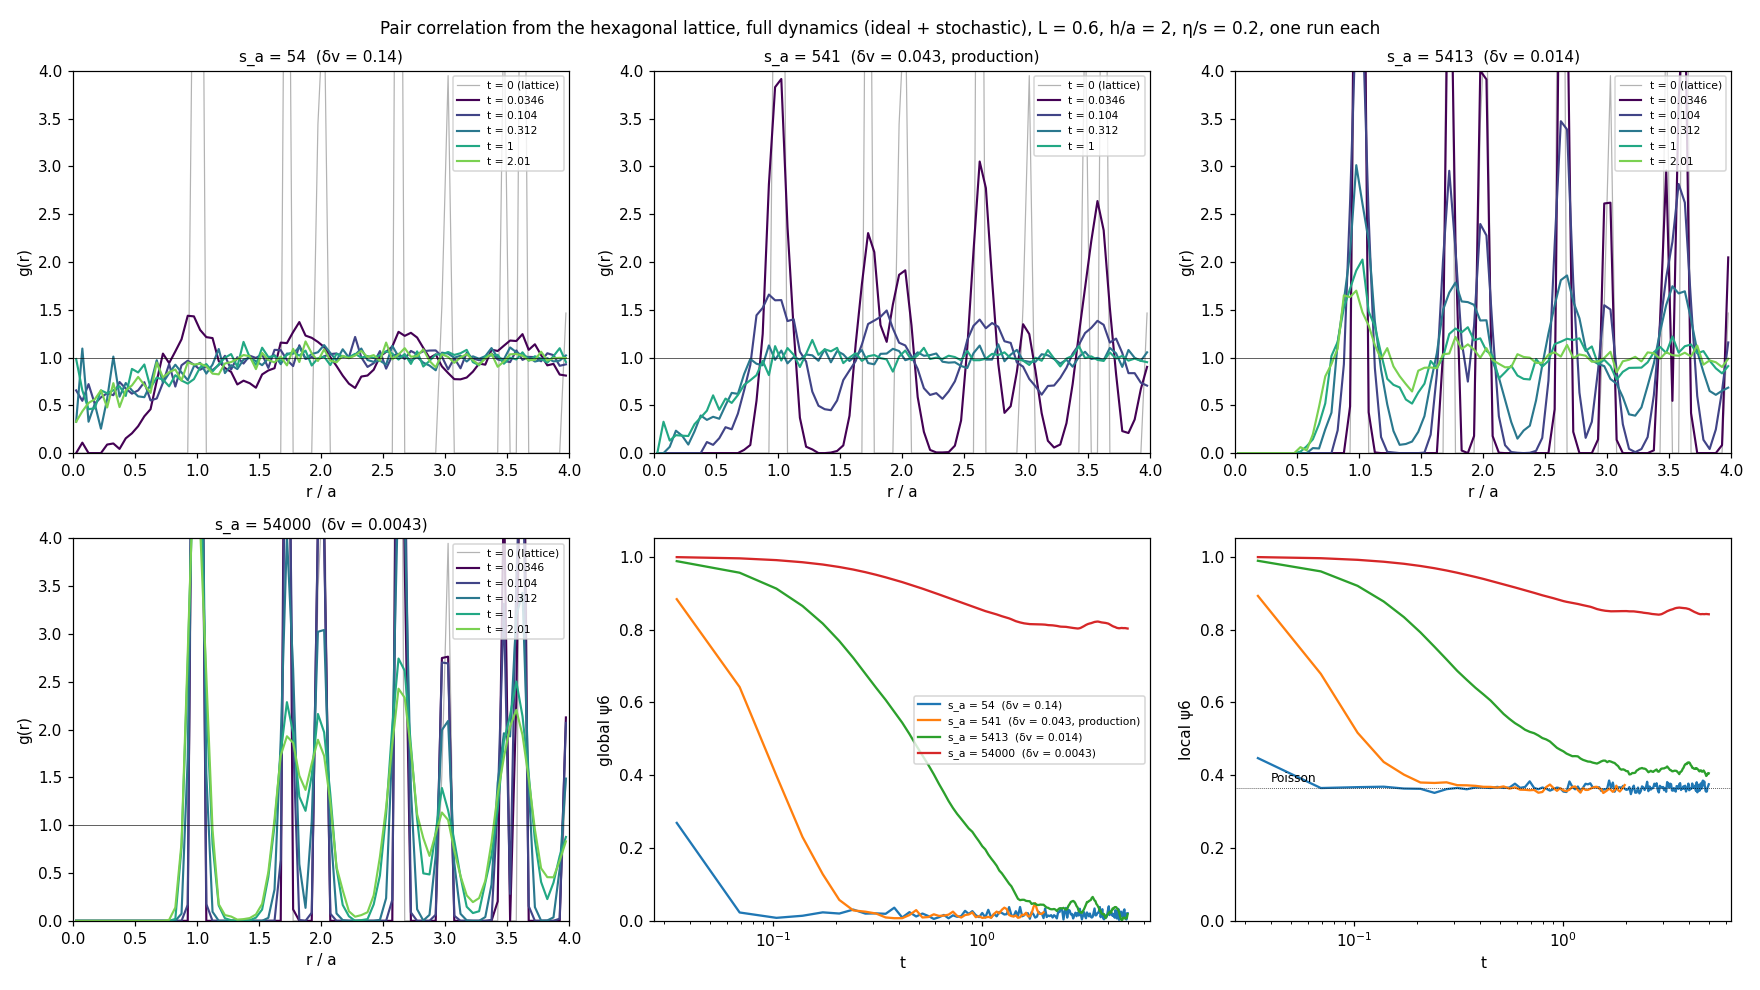
\includegraphics[width=\textwidth]{figs/equilibrium_g_vs_t.png}
\caption{The pair correlation from the hexagonal lattice, full dynamics, $L=0.6$, $h/a=2$, $\eta/s=0.2$, one run per entropy.
Panels 1--4: $g(r)$ at a sequence of times (grey: the lattice at $t=0$).  Panels 5, 6: global and local $\psi_6$ against time
(dotted: the local value for Poisson positions).}
\label{fig:gvt}
\end{figure}

%=============================================================================
\section{Hybrid Monte Carlo against the dynamics}
\label{sec:hmcvsdyn}

Stage 2 of \Sect{sec:plan} is implemented (\texttt{src/hmc.jl}, \texttt{test/testhmc.jl}, \texttt{examples/hmc\_positions.jl}).  On a box
of $N=168$ particles, a trajectory of ten steps followed by the trajectory with the momenta reversed returns to the start to
$10^{-13}$, and the energy error of a trajectory of fixed length falls as $\delta t^2$ (ratios $4.02$, $4.01$).  At $L=0.6$
($N=672$), with $\delta t$ half the acoustic step and ten steps per trajectory, the acceptance is $0.95$--$1.0$, the heat-bath
chains accept $58\%$ of their moves, and $600$ updates take about $20$ seconds.

\Fig{fig:hmcvsdyn} compares one chain of $600$ updates from the lattice (the second half averaged) with the late times of the
runs of \Fig{fig:gvt}, at the same $\beta^\mu$.  Hybrid Monte Carlo has no viscous step: its target \Eq{joint} involves only the
Hamiltonian and the equation of state, so the choice of viscous kernel enters only the dynamics.
\begin{itemize}
\item \emph{Short range: the two agree.}  $g(r)$ lies on top of the dynamics at all three entropies, and so does the local bond
  order:
  \st
  \psi_6^{\rm local}:\quad 0.367\ \text{vs}\ 0.361\ (s_a=541),\qquad 0.418\ \text{vs}\ 0.415\ (5413),\qquad 0.869\ \text{vs}\ 0.849\ (54000)
  \stp
  (HMC first).  The dynamics reaches the equilibrium local structure quickly.
\item \emph{Long wavelengths: they do not.}  The fluctuations of the number density of the positions at $kh=0.52$ and $0.74$ are
  lower in the dynamics, at every entropy,
  \st
  \frac{|N_{\bm k}|^2_{\rm dyn}}{|N_{\bm k}|^2_{\rm HMC}}=0.07\text{--}0.42 ,
  \stp
  while those of the entropy density $|S_{\bm k}|^2$ scatter about the same values (ratios $0.5$--$2.6$, single noisy runs).
\end{itemize}
A tentative reading.  The ideal step holds each $s_a$ fixed, so the way a long-wavelength fluctuation of the entropy density is
shared between the number of particles and the entropy per particle is frozen in from the start, and only the stochastic step
changes it, slowly.  Hybrid Monte Carlo redraws the $s_a$ at every update.  The dynamics runs reach only $t\le5$ in a small box;
campaign \texttt{pairs} ($t=200$, $L=1.2$) will show whether $|N_{\bm k}|^2$ of the dynamics climbs to the equilibrium value or
stays low.  If it stays low, the dynamics carries a long-wavelength non-equilibrium in the arrangement of the particles, to be
compared with the equal-time deficit of $C_{EE}$ along the flow (\texttt{commonkernel.tex}).

\begin{figure}[t]
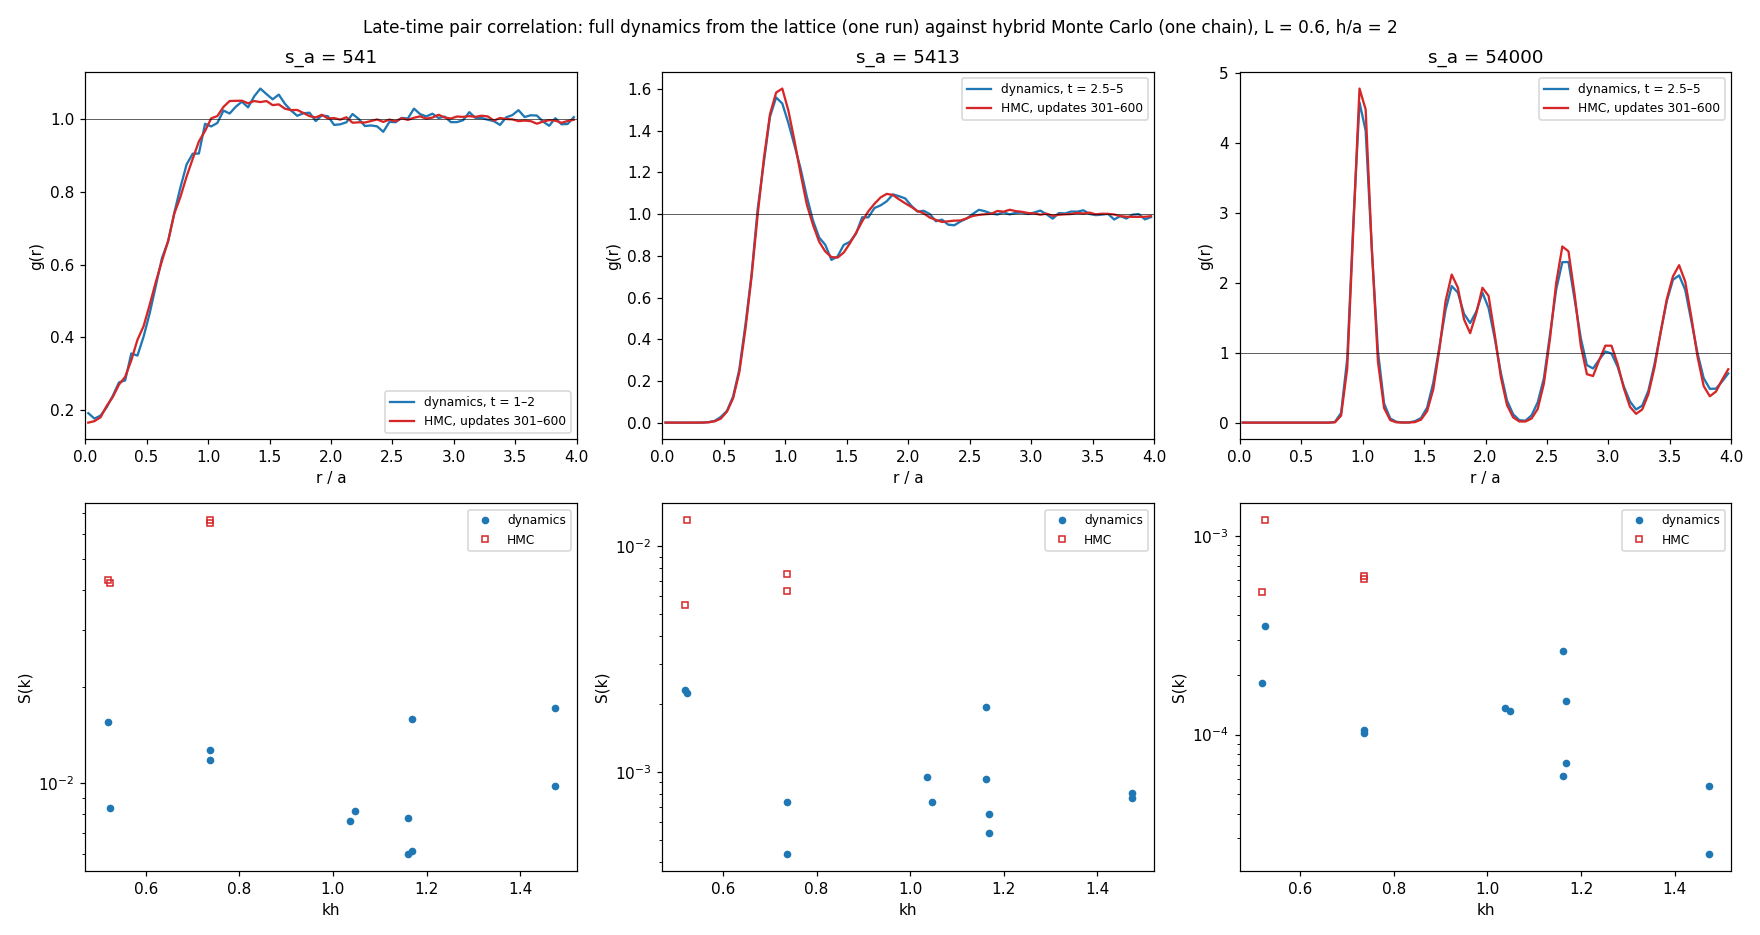
\includegraphics[width=\textwidth]{figs/equilibrium_hmc_vs_dynamics.png}
\caption{Late times of the full dynamics from the lattice (one run, the second half of $t\le2$ or $5$) against hybrid Monte
Carlo (one chain, updates $301$--$600$), $L=0.6$, $h/a=2$.  Top: $g(r)$.  Bottom: the structure factor of the positions,
$S(\bm k)=|N_{\bm k}|^2/N$ (the HMC chain records only $kh\le1$).}
\label{fig:hmcvsdyn}
\end{figure}

%=============================================================================
\section{Implementation plan}
\label{sec:plan}

Three stages, each usable on its own.  Nothing in the dynamics changes; the default runs stay bit-identical.

\paragraph{Stage 1: the pair correlation as a measurement.}  First, because it is cheap and immediately answers how the
positions relax from the lattice.
\begin{itemize}
\item \texttt{src/measure.jl}: extend \texttt{ParticleRecorder} with, at each record,
  \begin{itemize}
  \item $g(r)$ from the neighbour list (pairs within $2h$, the kernel support), in bins of $a/20$, normalized by the ideal-gas count;
  \item $g(r,\theta)$ in two angular bins, along and across the flow;
  \item $\psi_6$, over the six nearest neighbours of each particle;
  \end{itemize}
  and add the number density of the positions,
  \st
  N_{\bm k}=\sum_ae^{-i\bm k\cdot\bm x_a},
  \stp
  to \texttt{Recorder} at the wavevectors of the correlators, so $S(\bm k,t)=|N_{\bm k}|^2/N$.
\item \texttt{write\_equilibrium\_h5}: the datasets \texttt{part\_g}, \texttt{part\_g\_par}, \texttt{part\_g\_perp}, \texttt{part\_rbins},
  \texttt{part\_psi6}, \texttt{N}.
\item \texttt{examples/pair\_analysis.jl}: $g(r,t)$, $S(k,t)$ and $\psi_6(t)$ from a campaign.
\item Test: the lattice gives its shells exactly and $\psi_6=1$; Poisson positions give $g=1$ and $S=1$ within the noise.
\end{itemize}
\medskip
\noindent\fbox{\begin{minipage}{0.95\textwidth}
\textbf{Algorithm: pair observables} (at each record)
\begin{algorithmic}[1]
\State $g,\ g_\parallel,\ g_\perp\gets0$ in bins of $a/20$ up to $2h$
\For{each pair $a<b$ in the neighbour list} \Comment{pairs within $2h$}
  \State $\bm r_{ab}$ by the minimum image, $r=|\bm r_{ab}|$
  \State $g(r)\gets g(r)+2$
  \If{$|r_x|>|r_y|$} \State $g_\parallel(r)\gets g_\parallel(r)+2$ \Else \State $g_\perp(r)\gets g_\perp(r)+2$ \EndIf \Comment{flow along $x$}
\EndFor
\State \textbf{normalize}: divide each bin by $N\,n_0$ times the area of the shell, $n_0=N/A$ \Comment{ideal-gas count}
\For{each particle $a$}
  \State \textbf{bond order}: six nearest $b$, $q_a=\frac16\sum_be^{6i\theta_{ab}}$, $\theta_{ab}$ the angle of $\bm r_{ab}$ to $x$
\EndFor
\State $\psi_6\gets\big|\sum_aq_a\big|/N$
\For{each wavevector $\bm k$ of the correlators}
  \State $N_{\bm k}\gets\sum_ae^{-i\bm k\cdot\bm x_a}$ \Comment{$S(\bm k,t)=|N_{\bm k}|^2/N$}
\EndFor
\end{algorithmic}
\end{minipage}}
\medskip


\paragraph{Stage 2: hybrid Monte Carlo.}  \texttt{src/hmc.jl} (new).
\begin{itemize}
\item \emph{Heat bath} at fixed $\beta^\mu$: for each particle a few steps of the independence Metropolis chain of
  \texttt{draw\_particle}, \emph{started from its current} $(e_a,\bm m_a)$, so that the conditional distribution is preserved
  exactly (a fresh chain of finite length is only approximately exact); then $s_a=S_a(e_a,\bm m_a)$.  $\beta^\mu$ is fixed for the
  whole sampling, set once from the target state; the totals are not shifted.
\item \emph{Generalized leapfrog} (\Sect{sec:sampler}) with the present force (\texttt{hamiltonian\_force\_energy!}) and velocities;
  the implicit half steps iterated to a tolerance of $10^{-12}$, so that the step is reversible to that accuracy.
\item \emph{Acceptance}: $H$, $\bm P$ and $\prod_aT_a$ at both ends of the trajectory; on rejection the positions and momenta are
  restored.
\item Parameters: the number of updates, the leapfrog steps per trajectory, and $\delta t$ as a fraction of the acoustic step;
  the acceptance is reported (aim: $0.7$--$0.9$).
\item \texttt{examples/equilibrium.jl}: \texttt{SR\_POSITIONS=hmc} with \texttt{SR\_HMC\_N}, \texttt{SR\_HMC\_STEPS}, \\
  \texttt{SR\_HMC\_DTFAC}: the given number of updates from the lattice, recorded with the stage-1 observables, then the present
  start (\texttt{SR\_START=eq}, totals shifted exactly) and the run.  Not with the grid ideal step, whose positions are fixed.
\end{itemize}
\medskip
\noindent\fbox{\begin{minipage}{0.95\textwidth}
\textbf{Algorithm: one update of hybrid Monte Carlo} at the fixed target $\beta^0=1/T$, $\bm\beta=\bm v/T$, measure $\pi_E$
\begin{algorithmic}[1]
\For{each particle $a$} \Comment{heat bath at fixed positions}
  \State continue the Metropolis chain of \texttt{draw\_particle} for a few steps from the current $(e_a,\bm m_a)$, at volume $V_a$
  \State $s_a\gets S_a(e_a,\bm m_a)$
\EndFor
\State \textbf{save} $\{\bm x_a,\bm m_a\}$ and $H_0=H$, $\bm P_0=\sum_a\bm m_a$, $\Lambda_0=\sum_a\ln T_a$
\For{each of the leapfrog steps} \Comment{generalized leapfrog, $s_a$ fixed}
  \Repeat \Comment{positions fixed: equation of state and force only}
    \State $\bm m^{1/2}\gets\bm m-\tfrac{\delta t}2\,\partial H/\partial\bm x\,(\bm x,\bm m^{1/2})$
  \Until{the change is below $10^{-12}$}
  \Repeat \Comment{each pass smooths at the new positions}
    \State $\bm x'\gets\bm x+\tfrac{\delta t}2\big[\bm v(\bm x,\bm m^{1/2})+\bm v(\bm x',\bm m^{1/2})\big]$
  \Until{the change is below $10^{-12}$}
  \State $\bm m\gets\bm m^{1/2}-\tfrac{\delta t}2\,\partial H/\partial\bm x\,(\bm x',\bm m^{1/2})$, \quad $\bm x\gets\bm x'$
\EndFor
\State $\Delta\ln\pi\gets-\beta^0(H-H_0)+\bm\beta\cdot(\bm P-\bm P_0)+\big(\sum_a\ln T_a-\Lambda_0\big)$
\If{$\ln u\ge\Delta\ln\pi$, $u$ uniform in $(0,1)$} \State \textbf{reject}: restore the saved $\{\bm x_a,\bm m_a\}$ \EndIf
\end{algorithmic}
\end{minipage}}
\medskip

$\partial H/\partial\bm x$ is minus the present force (\texttt{smooth\_to\_particles!}, \texttt{update\_thermodynamics!},
\texttt{hamiltonian\_force\_energy!}); $\bm v$ are the particle velocities of the same pass.

In the driver (\texttt{SR\_POSITIONS=hmc}): set up the lattice; take $\beta^\mu$ from the target state; make \texttt{SR\_HMC\_N}
updates, recording the stage-1 observables, the acceptance and $H$; then the present start (\texttt{SR\_START=eq}, totals
shifted exactly) and the run as now.

Tests (\texttt{test/testhmc.jl}):
\begin{enumerate}
\item \emph{Reversibility}: a trajectory, then the trajectory from the end with the momenta reversed, returns to the start
  to $10^{-10}$.
\item \emph{Volume preservation}: the Jacobian of one leapfrog step on a small system, by finite differences, has
  determinant 1.
\item \emph{Energy error} of a trajectory scales as $\delta t^2$.
\item \emph{Two samplers agree}: on a small box, the distribution of the volumes and $g(r)$ from hybrid Monte Carlo against
  single-particle Metropolis moves with \Eq{Px}.
\end{enumerate}

\paragraph{Stage 3: the runs of \Sect{sec:runs}} at NERSC, with a node-hour estimate before submitting.

\paragraph{Branch.}  \texttt{equilibrium}, off \texttt{common-default}; stage 1 can go to \texttt{main} on its own.

\end{document}
